\documentclass[border=3pt,tikz]{standalone}
% Shared look for every TikZ figure in these notes.
% Included by each standalone figure file; also keeps the figures consistent
% with the colours used in the PDF and on the website.

\usepackage{tikz}
\usepackage{pgfplots}
\pgfplotsset{compat=1.18}
\usetikzlibrary{arrows.meta, decorations.markings, decorations.pathmorphing,
                patterns, calc, positioning}
\usepackage{amsmath}

% Series colours are the three validated categorical slots also used by the
% interactive widgets, so a path drawn in the printed notes and the same path on
% the website are the same colour. They clear the colour-vision-deficiency and
% contrast checks as a set; every path is direct-labelled as well, so colour is
% never the only thing carrying identity.
\definecolor{duPurple}{HTML}{68246D}
\definecolor{duBlue}{HTML}{2A78D6}
\definecolor{duRed}{HTML}{EB6834}
\definecolor{duGreen}{HTML}{1BAF7A}
\definecolor{duGrey}{HTML}{6B6B6B}

\tikzset{
  axisline/.style   = {-{Stealth[length=3mm]}, line width=0.7pt, black},
  path1/.style      = {duBlue,   line width=1.1pt},
  path2/.style      = {duRed,    line width=1.1pt},
  path3/.style      = {duGreen,  line width=1.1pt},
  statedot/.style   = {circle, fill=black, inner sep=1.4pt},
  arrowhead/.style  = {decoration={markings,
                        mark=at position #1 with {\arrow{Stealth[length=2.6mm]}}},
                       postaction={decorate}},
  lbl/.style        = {font=\small},
  slbl/.style       = {font=\footnotesize, duGrey},
  workfill/.style   = {duPurple, opacity=0.16},
}

\begin{document}
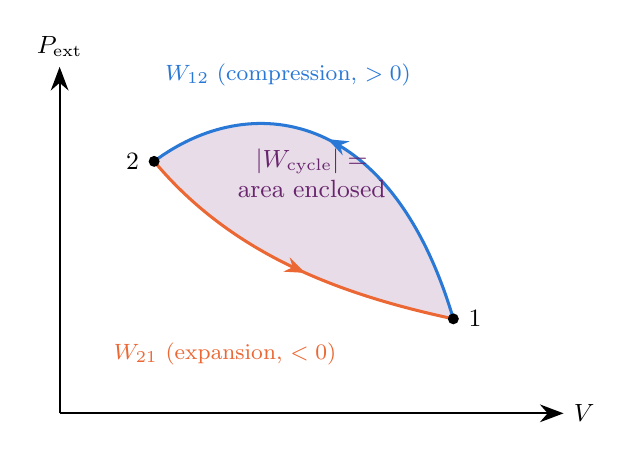
\begin{tikzpicture}[scale=1]
  \draw[axisline] (0,0) -- (6.4,0) node[right, lbl] {$V$};
  \draw[axisline] (0,0) -- (0,4.4) node[above, lbl] {$P_\text{ext}$};

  \coordinate (s1) at (5.0,1.2);
  \coordinate (s2) at (1.2,3.2);

  \fill[workfill]
    (s1) .. controls (4.2,3.9) and (2.4,4.1) .. (s2)
         .. controls (2.2,2.0) and (3.6,1.5) .. (s1) -- cycle;

  \draw[path1, arrowhead=0.55] (s1) .. controls (4.2,3.9) and (2.4,4.1) .. (s2);
  \draw[path2, arrowhead=0.55] (s2) .. controls (2.2,2.0) and (3.6,1.5) .. (s1);

  \node[statedot] at (s1) {}; \node[lbl, right=2pt] at (s1) {1};
  \node[statedot] at (s2) {}; \node[lbl, left=2pt]  at (s2) {2};

  \node[lbl, duPurple, align=center] at (3.2,3.05)
    {$|W_\text{cycle}|$ =\\area enclosed};
  \node[slbl, duBlue] at (2.9,4.3) {$W_{12}$ (compression, $>0$)};
  \node[slbl, duRed]  at (2.1,0.75) {$W_{21}$ (expansion, $<0$)};
\end{tikzpicture}
\end{document}
